\documentclass{article}
\usepackage{graphicx} % Required for inserting images
\usepackage{amsmath}
\usepackage{tikz}
\usetikzlibrary{arrows.meta}
\title{Factibilidade monetária de um equilíbrio geral}
\author{Marcelo Fiorelli}
\date{October 2025}

\begin{document}

\maketitle
\section{Introdução}
\par Este arquivo serve para proteger uma ideia. Essa ideia pode não ser originalmente minha. Trata-se da estruturação do problema de factibilidade monetária em rede de uma economia em equilíbrio geral, um rascunho da demonstração de que um equilíbrio geral é sempre monetariamente factível, e uma possível classe de modelos novos de iliquidez e desequilíbrio.

\section{O Problema: Matriz de Transações e Equilíbrio Geral}
\par Em uma determinada economia, todas as transações econômicas em um período arbitrário podem ser representadas por um grafo com pesos e direcionado:

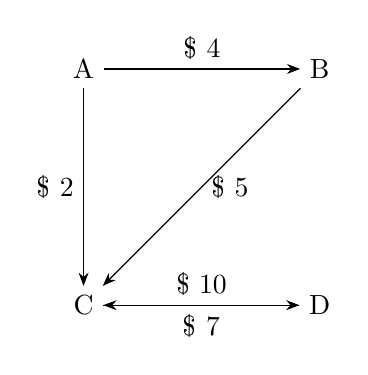
\begin{tikzpicture}[
    >=Stealth,              % arrow tip style
    node distance=3cm,      % spacing between nodes
    node/.style={circle, draw, minimum size=1cm}]
    % Nodes
    \node (A) {A};
    \node (B) [right of=A] {B};
    \node (C) [below of=A] {C};
    \node (D) [right of=C] {D};

    % Directed edges with weights
    \draw[->] (A) -- node[midway, above] {\$ 4} (B);
    \draw[->] (A) -- node[midway, left] {\$ 2} (C);
    \draw[->] (B) -- node[midway, right] {\$ 5} (C);
    \draw[->] (D) -- node[midway, above] {\$ 10} (C);
    \draw[->] (C) -- node[midway, below] {\$ 7} (D);
\end{tikzpicture}

\par Se os agentes utilizam somente uma única moeda como meio de troca (i.e., o meio de pagamento legalmente determinado em um país), e se ignorarmos o lado real das transações (i.e., bens, serviços, ativos e passivos), temos a rede de transações ou a rede de fluxos de uma economia em dado período. Esse grafo pode ser representado por uma matriz de adjacência, que será chamada de matriz de transações ou matriz de fluxos. 

$$ A =
\begin{bmatrix}
 0&     a_{1,2}   &    \cdots    & a_{1,n} \\
 a_{2,1} & 0     &        &  \vdots \\
 \vdots &        & \ddots & \vdots  \\
a_{n,1} &   \cdots     &   \cdots     & 0
\end{bmatrix}
$$

\par Nessa matriz, a célula $a_{i,j}$ indica o valor monetário saindo do bolso do indivíduo/firma $i$ e indo para o bolso do indivíduo/firma $j$. Assim, se somarmos todos os valores da linha $i$, temos o total de saídas do caixa de $i$, e se somarmos todos os valores da linha $j$ temos o total de entradas do caixa de $j$. Por convenção, vamos estabelecer que não existe auto-transferência (auto-loop), e não existe transferência negativa (todas as entradas da matriz são positivas). Um valor $a_{i,j}$ negativo pode simplesmente ser representado por um valor $a_{j,i}$ de mesmo valor absoluto mas positivo, sem perda de sentido.
\par Se tivermos um vetor de dotações monetárias, podemos computar, a partir da matriz de transações, como ficam as dotações monetárias após todas as transações do período. Basta, para cada indivíduo, somar as entradas e subtrair as saídas. Assim, temos a fórmula:
$$ w_0 = (w^1_0, \cdots, w^n_0)'$$
$$w_1 = (\sum^n_{j=1}{a_{j,i}} -\sum^n_{j=1}{a_{i,j}}  )^n_{i=1}+w_0$$
\par Note que se somarmos todas as coordenadas do vetor $w_1$ (o que inclusive seria um norma soma, nesse caso), estaríamos basicamente somando todos os valores da matriz no primeiro termo, no segundo termo estaríamos também somando todos os valores da matriz, e no terceiro termo estaríamos somando todos os valores de $w_0$. Logo, qualquer matriz de transações sempre preservará o estoque de moeda de uma economia. Essa é uma limitação clara do nosso arcabouço teórico que obrigará sua reformulação no futuro. Mas estamos justamente tentando avaliar o que acontece quando o estoque monetário é fixo, portanto, essa é uma propriedade fundamental do nosso modelo.
\par Note também que a matriz de transações é algo que existe no "mundo real". Esse problema de estoque monetário fixo surge pois não incluímos transações com o Banco Central nem com o Tesouro no nosso modelo. Mas a matriz de transações existe, por mais que não consigamos observar ela, já que muitas transações acontecem em dinheiro, ou não pagam imposto, ou simplesmente por se tratar de um volume muito grande de transações.
\par Nada do que foi dito até agora é nenhuma novidade. E talvez nem o que venha logo a seguir: para cada alocação e vetor de preços de equilíbrio, existe pelo menos uma matriz de transações que a representa. 
\par Se temos uma alocação de equilíbrio, cada indivíduo e firma apresenta uma função demanda por bens e serviços, cada indivíduo e firma apresenta uma oferta de bens e serviços, e existe um subespaço de vetores de preços $p$ tal que:

$$ \sum^{n}_{i}x^l_i(p) = \sum^n_{i} y^l_i(p)$$

\par Sendo $x^l_i(p)$ a demanda do indivíduo/firma $i$ pelo bem $l$, e $y^l_i(p)$ a oferta do bem $l$ pelo indivíduo/firma $i$. Note que aqui equilibramos oferta e demanda a partir de mercados de bens homogêneos, e não a partir de transações entre indivíduos/firmas. Ou seja, um mesmo indivíduo pode saciar sua demanda pelo bem $l$ comprando tudo que deseja da firma A, ou da firma B, ou de uma combinação das duas, ou de uma combinação de todos os indivíduos e firmas que ofertam o bem $l$. Realmente, se somente uma firma ofertar o bem $l$, ou então somente um consumidor demandar o bem $l$, só há um conjunto de transações que sacia essa demanda. Agora, se tivermos $n'>1$ consumidores e $n''>1$ ofertantes do bem $l$, teremos infinitos conjuntos de transações possíveis que equilibram o mercado do bem $l$. 

\par Portanto, um único equilíbrio geral pode gerar infinitas possibilidades de transações monetárias. Mas cabe, finalmente, a pergunta (o "pulinho" do gato): dado um conjunto de transações monetárias realizado por um equilíbrio geral, essas transações monetárias são possíveis dado uma dotação monetária?

\par Mas ai cabe uma outra pergunta: como a moeda entra nesse modelo? Podemos incluir a moeda em um arcabouço de equilíbrio geral com fluxos monetários? Temos duas possibilidades: 1) Não há demanda por moeda; 2) Há demanda por moeda. 

\par Se considerarmos que não existe demanda por moeda, mas ela é necessária para as trocas (sem ela, as trocas não ocorrem), precisamos descobrir se dado um vetor dotação monetária não nulo se é possível realizarmos subtransações até que todas as transações delimitadas pela matriz de transações se esgotem.

\par Por subtransações queremos dizer que em uma rodada de trocas, os indíviduos realizam transações sem ultrapassar seu estoque monetário (ou seja, sem caixa negativo), mas também sem realizar mais trocas do que precisam. Há medida que as trocas ocorrem e as rodadas se passam, os indivíduos adquirem mais moedas em caixa e podem realizar as transações que ainda desejam realizar. 

\par Assim, primeiro definimos uma matriz de subtransação ou subfluxo:

$$ S_{t+1} := [s^{t+1}_{i,j}:(\forall(i,j), s^{t+1}_{i,j} \leq a^t_{i,j}) \land (\forall i, \sum^n_{j} s^{t+1}_{i,j} \leq w^i_t)]_{n \times n} $$

\par Ou seja, uma matriz de subtransação é uma matriz de transações possíveis dado o estoque monetário dos agentes em um subperíodo $t$ e as transações planejadas do período total. Note que $w_t$ é atualizado de acordo com o perído a partir da equação:

$$w_{t} = (\sum^n_{j=1}{s^{t}_{j,i}} -\sum^n_{j=1}{s^t_{i,j}}  )^n_{i=1}+w_{t-1}$$

\par Portanto, queremos saber para quais matrizes de transação $A$, existe $w_0$ para o qual seja possível esgotar todas as transações a partir de uma sequência finita $\{S_k\}^m_{k=1}$ de subtransações.
\par Assim, a condição fraca de factibilidade do par $(w_0, A)$ seria: $A$ e $w_0$ são factíveis se existe $\{S_k\}^m_{k=1}$ tal que:
$$ A = \sum^m_{k=1} S_k$$
\par Ou:
$$ A - \sum^m_{k=1} S_k = 0$$
\par Apesar da longa explicação, esse problema não é tão interessante. Sabemos que se a matriz de transferência não for fortemente conectada, para algumas dotações não é possível a moeda sair de uma comunidade e chegar na outra, portanto o par matriz e dotação não é factível. Mas para qualquer região fortemente conectada com dotação não nula, muito provavelmente sempre existe solução, desde que, para todo $i$:
$$\sum^n_{j=1}{a_{j,i}} = \sum^n_{j=1}{a_{i,j}}  $$
\par Ou seja, as entradas devem ser iguais as saídas. Isso não é um problema para uma solução de equilíbrio geral sem demanda por moeda, já que essa já é uma propriedade desse problema (é fácil mostrar, a partir da restrição orçamentária dos consumidores que a soma das linhas é igual a soma das colunas).
\par O problema se torna mais interessante quando estamos tratando de um modelo de equilíbrio geral com demanda por moeda. Se há demanda por moeda, a moeda aparece na função utilidade, ou seja, trata-se de um modelo \textit{Money in Utility} (MIU). Nesse caso, não basta que a moeda realize todas as transações. Devemos satisfazer o equilíbrio parcial:
$$ \sum^{n}_{i}x^m_i(p) = \sum^n_{i} y^m_i(p)$$
\par Sendo $x^m_i$ a demanda do indivíduo $i$ por moeda e $y^m_i$ a oferta do indivíduo $i$ de moeda. Como nenhuma firma produz moeda, temos:
$$ \sum^{n}_{i}x^m_i(p) = \sum^n_{i} e^m_i$$
\par Sendo $e^m_i$ a dotação de moeda do indivíduo $i$, que na verdade denotamos aqui como $w^i_0$. Após concluídas as transações, temos $x^m_i = w^i_T$.
\par Agora, portanto, nosso problema de factibilidade monetária mudou. Não basta a moeda circular, esgotando todas as transações planejadas. Ela precisa também "parar" no lugar certo, com a pessoa certa, depois de realizar todas as trocas necessárias.
\par Assim, a condição forte de factibilidade do trio $(w_0, w_T,  A)$, em que $|w_0| = |w_T|$ seria: $A$, $w_0$  e $w_T$ são factíveis se $$w_T = (\sum^n_{j=1}{a_{j,i}} -\sum^n_{j=1}{a_{i,j}}  )^n_{i=1}+w_0$$
\par e se existe $\{S_k\}^m_{k=1}$ tal que:
$$ A = \sum^m_{k=1} S_k$$
\par Esse não é um problema trivial. Mas creio que consigo provar que se a matriz $A$ é fortemente conectada e a primeira condição de factibilidade é satisfeita, então a segunda condição também é satisfeita sempre. Então segue um rascunho do teorema e um rascunho de sua demonstração:
\par \textbf{Teorema:} Para toda matriz $A$ fortemente conectada e todo par de vetores $w_T$ e $w_0$ tal que $w_T = (\sum^n_{j=1}{a_{j,i}} -\sum^n_{j=1}{a_{i,j}}  )^n_{i=1}+w_0$, o trio $(w_0, w_T, A)$ é factível. Ou seja, existe $\{S_k\}_{k=1}^m$ tal que:
$$ A = \sum^m_{k=1} S_k$$
Sendo $S_k$ da forma:
$$ S_{k} := [s^{k}_{i,j}:(\forall(i,j), s^{k}_{i,j} \leq a^{k-1}_{i,j}) \land (\forall i, \sum^n_{j} s^{k}_{i,j} \leq w^i_{k-1})]_{n \times n} $$
\par \textbf{Demonstração:} Para essa demonstração (rascunho), uma argumentação baseada em grafos é mais promissora do que uma argumentação baseada em álgebra matricial.
\par Suponha, por contradição, que não é factível. Suponha, além disso, que já realizamos o máximo de transações possíveis, e chegamos no último dos estados finais. Isso significa que todos os nós que demandam moeda ($w^i_t>0$) já realizaram todas as suas transações. Caso contrário, não estamos no último estado. As transações que restam são aquelas de nós que não têm moeda.
\par Note que para toda transação feita, temos a condição:
$$w^i_t = \sum^n_{j=1} {s^t_{j,i}}-\sum^n_{j=1} {s^t_{i,j}} + w^i_{t-1}$$
\par Ou então, se combinarmos várias matrizes de subtransação:
$$w^i_t = \sum^n_{j=1} {s^t_{j,i}}-\sum^n_{j=1} {s^t_{i,j}} + w^i_{0}$$
\par Todos os nós que completaram suas transações estão com a quantidade demandada de moeda. Caso contrário, se tivessem moeda de mais, significaria que $w^i_T < w^i_t$ o que implica ou que foram feitas compras de menos (o que implica que o indivíduo ainda pode fazer compras) ou vendas de mais (o que implica que o indivíduo realizou vendas que não desejava fazer). 
\par Já no cenário em que $w^i_T > w^i_t$, vamos supor, inicialmente que o nó $A$ realizou todas as suas compras e tem uma quantidade positiva de moeda, mas que seja inferior a quantidade demandada. Isso implica a existência de outro nó B, com zero moeda em estoque, mas que deseja realizar compras com A. Todavia, para ser capaz de realizar essas compras, o nó B precisa ter um volume de vendas maior ou igual ao volume de compras que realiza com A e demais nós. Se seguirmos esse processo indutivamente, chegamos a conclusão que tal cenário só é possível se existir pelo menos um indivíduo que deseja realizar compras e tem estoque de moeda (o que contradiz nossa suposição de estado final) ou se existir um indivíduo que deseja realizar compras mas não tem moeda (o que contradiz a hipótese de consistência do caixa). Portanto, o único estado final possível é aquele em que $w^i_T = w^i_t$, e não só isso, mas o vetor inteiro é satisfeito: $w_T = w_t$, já que caso haja alguma comunidade com estoque de moeda e transações a serem feitas ainda, não estamos no estado final.
\par Portanto, a possibilidade de "existência de não factibilidade" seria em comunidades que não apresentam demanda líquida por moeda. Nosso estado é da seguinte forma:
\par \begin{tikzpicture}[
    >=Stealth,              % arrow tip style
    node distance=3cm,      % spacing between nodes
    node/.style={circle, draw, minimum size=1cm}]
    % Nodes
    \node (A) {A};
    \node (B) [right of=A] {B};
    \node (C) [below of=A] {C};
    \node (D) [right of=C] {D};
    \node (E) [right of = B] {E};
    \node (F) [right of = E] {F};
    \node (G) [below of = E] {G};
    \node (H) [below of = F] {H};

    % Directed edges with weights
    \draw[->] (B) -- node[midway, above] {\$ 2} (A);
    \draw[->] (A) -- node[midway, left] {\$ 2} (C);
    \draw[->] (B) -- node[midway, right] {\$ 5} (C);
    \draw[->] (D) -- node[midway, above] {\$ 3} (C);
    \draw [->] (D) -- node[midway, right] {\$ 7} (B);
    \draw[->] (C) -- node[midway, below] {\$ 10} (D);
\end{tikzpicture}
\par Em que E, F, G e H apresentam algum estoque de moeda, em quanto A, B, C e D não apresentem nenhum estoque de moeda.
\par Suponha, sem perda de generalidade, que as matrizes de subtransação contenham uma transação cada. Se revertermos as transações uma por uma, há duas possibilidades:
\par 1) Não existiam transações entre a comunidade com moeda (representada na figura pelas letras de E a H) e a comunidade sem moeda (representada pelas letras de A a D). Isso por sua vez implica que a matriz A não é fortemente conectada (contradição!);
\par 2) Existiam transações entre as duas comunidades, mas a moeda "entrou e saiu rapidamente".
\par Para o segundo caso, temos uma situação parecida com o problema sem demanda por moeda. Uma solução para esse problema pode servir nessa etapa da demonstração. Todavia, não é necessário. Basta observar que a partir dessa etapa, se existirem mais de dois nós na comunidade sem moeda (o que implica existirem no mínimo duas transações), podemos sempre realizar pelo menos uma transação a mais do que foi feito. Ou seja, chegamos em um estado final anteriormente, mas ele não é o último estado final. Nunca poderíamos chegar ao último estado final que não seja o esgotamento completo de todas as transações.
\par Mas e se não há último estado final? Ou seja, e se pudermos sempre a chegar a um estado como esse de comunidades sem moeda? Essa é uma hipótese pouco plausível, mas que não consigo demonstrar ainda porque seria impossível. A verdade é que podemos sim realizar uma soma convergente de matrizes $S_k$ que não esgota a matriz $A$. Mas creio que o fato de, caso você caia nesse caso de "estado armadilha", você pode sempre voltar atrás e refazer as transações de maneira a completar mais transações, e o fato de o problema sem demanda por moeda ter solução pra qualquer dotação não nula, faz com que nós tenhamos uma solução finita para nosso problema. Portanto, termino aqui esse rascunho de demonstração.
\par Assim, concluímos que um equilíbrio geral MIU é sempre monetariamente factível. Mas o que esse resultado significa? Significa basicamente que se os agentes decidem os preços no começo do período de modo a garantir o equilíbrio, e se os agentes planejam suas transações, todas as transações planejadas serão possíveis de serem realizadas, desde que em uma ordem correta. Isso não diz nada sobre quantas transações serão necessárias para que isso ocorra.
\par Esse, por si só, é um resultado bastante útil no fortalecimento do conceito de equilíbrio geral, apesar de vários problemas práticos. É uma porta de entrada para discutirmos problemas mais complexos envolvendo tempo de transações, velocidade da moeda, desutilidade intertemporal, endogeneidade da moeda etc.
\section{Um modelo de "armadilha da moeda"}
\par A partir do que discutimos na seção anterior, vimos que se as transações forem feitas na ordem errada, podemos criar comunidades em que as demandas por moeda são saciadas, mas nenhuma transação é desejada de ser realizada, e comunidades em que deseja-se transacionar, mas não há moeda. Ou seja comunidades com moeda e sem troca, e comunidades com desejo pela troca mas sem moeda. Situações em que comunidades inteiras demandam liquidamente exatamente "zero" unidades monetárias pode parecer algo que quase certamente não ocorrerá, o que é verdade. Mas note que algo próximo disso já é uma situação "problemática" do ponto de vista de se atingir o equilíbrio. Se a demanda líquida por moeda for muito próxima de zero em uma comunidade, pode ser que somente uma pequena quantidade de moeda entre na comunidade, fazendo com que seja necessário um número muito grande de transações para se atingir a alocação de equilíbrio.
\par Então, a ideia aqui proposta é justamente modelar como trocas em ordens aleatórias podem gerar uma situação de iliquidez. Qual a probabilidade de cairmos em uma região próxima da "armadilha da moeda"? O que ocorre com a velocidade de circulação da moeda?  Isso aumenta a preferência por moeda endogenamente? Essas situações de iliquidez promovem uma demanda maior por crédito comercial?
\end{document}
